%%%%%%%%%%%%%%%%%%%%%%%%%%%%%%%%%%%%%%%%%%%%%%%%%%%%%%%%%%%%%%%%%%%%%%%%%%%%%%%%
%2345678901234567890123456789012345678901234567890123456789012345678901234567890
%        1         2         3         4         5         6         7         8
\documentclass[letterpaper, 10 pt, conference]{ieeeconf} 
\usepackage{graphicx}
\usepackage{microtype}
\usepackage{ragged2e}
% Comment this line out if you need a4paper

%\documentclass[a4paper, 10pt, conference]{ieeeconf}      % Use this line for a4 paper

\IEEEoverridecommandlockouts                              % This command is only needed if 
                                                          % you want to use the \thanks command

\overrideIEEEmargins                                      % Needed to meet printer requirements.

%In case you encounter the following error:
%Error 1010 The PDF file may be corrupt (unable to open PDF file) OR
%Error 1000 An error occurred while parsing a contents stream. Unable to analyze the PDF file.
%This is a known problem with pdfLaTeX conversion filter. The file cannot be opened with acrobat reader
%Please use one of the alternatives below to circumvent this error by uncommenting one or the other
%\pdfobjcompresslevel=0
%\pdfminorversion=4

% See the \addtolength command later in the file to balance the column lengths
% on the last page of the document

% The following packages can be found on http:\\www.ctan.org
%\usepackage{epsfig} % for postscript graphics files
%\usepackage{mathptmx} % assumes new font selection scheme installed
%\usepackage{times} % assumes new font selection scheme installed
\usepackage{amsmath} % assumes amsmath package installed
\usepackage{tikz}
\usetikzlibrary{arrows.meta, positioning, fit, backgrounds, calc}
\usepackage[portuguese]{babel}
\addto\captionsportuguese{\renewcommand{\abstractname}{Abstract}}
\addto\captionsportuguese{\renewcommand{\refname}{References}}
%\usepackage{amssymb}  % assumes amsmath package installed
\setlength{\emergencystretch}{3em}

\title{\LARGE \bf
Identificação de Sistema e Modelagem de um Veículo Aéreo Não Tripulado (VANT) VTOL Híbrido modo Quadricóptero.
}


\author{$1^{st}$ Henrique Mark dos Santos Corrêa% <-this % stops a space
\\
\textit{Departamento de Engenharia Eletrônica (IEE)} \\
\textit{Instituto Tecnológico de Aeronáutica (ITA)} \\
São José dos Campos, Brazil \\
\tt\small henriquecorrea@ita.br
\and
$2^{nd}$ Neusa Maria Franco de Oliveira, Ph.D.\\
\textit{Departamento de Engenharia Eletrônica (IEE)} \\
\textit{Instituto Tecnológico de Aeronáutica (ITA)} \\
São José dos Campos, Brazil \\
\tt\small neusa@ita.br
}

\begin{document}

\maketitle
\thispagestyle{empty}
\pagestyle{empty}

%%%%%%%%%%%%%%%%%%%%%%%%%%%%%%%%%%%%%%%%%%%%%%%%%%%%%%%%%%%%%%%%%%%%%%%%%%%%%%%%
\begin{abstract}
O presente trabalho descreve a identificação de sistema e a validação de um modelo matemático não-linear para o modo de voo quadricóptero de um Veículo Aéreo Não Tripulado (VANT) VTOL de configuração híbrida. O objetivo principal é obter um modelo identificado do modo quadricóptero que sirva como base para o desenvolvimento de algoritmos de controle e de um piloto automático (PA) para as fases de decolagem e pouso vertical. A metodologia de identificação de sistemas M4V (Maneuver, Measurements, Methods, Models) foi aplicada, utilizando dados coletados em voos reais. Para estimar os parâmetros de inércia e os coeficientes aerodinâmicos, empregou-se um método de otimização por mínimos quadrados não-lineares no domínio do tempo, que minimiza o erro entre a resposta simulada e os dados medidos em manobras que excitaram os modos da aeronave. O modelo identificado foi validado comparando-se suas respostas com um conjunto distinto de dados de voo não utilizado na estimação. Os resultados demonstram boa correlação entre os dados reais e simulados, confirmando a adequação do modelo para as aplicações de controle pretendidas.

\textit{Keywords—} VTOL, Identificação de Sistemas, Quadricóptero, OEM
\end{abstract}


%%%%%%%%%%%%%%%%%%%%%%%%%%%%%%%%%%%%%%%%%%%%%%%%%%%%%%%%%%%%%%%%%%%%%%%%%%%%%%%%
\section{INTRODUÇÃO}

Veículos aéreos não tripulados (VANTs) com capacidade de decolagem e pouso vertical (VTOL, do inglês \textit{Vertical Take-off and Landing}) têm ganhado destaque devido à sua versatilidade, combinando a eficiência de cruzeiro de uma aeronave de asa fixa com a flexibilidade operacional de um multirotor [1]. A aeronave objeto deste estudo, o DH Hybrid-Drone VTOL, é um VANT de configuração híbrida capaz de transitar entre o modo de voo quadricóptero e o modo de asa fixa. A Figura~\ref{fig:fases_voo} ilustra as fases típicas de voo desse tipo de aeronave, desde a decolagem vertical até o pouso, passando pela transição e pelo cruzeiro como asa fixa.

Embora a aeronave opere em múltiplos modos de voo, as fases de decolagem e pouso vertical são realizadas exclusivamente no modo quadricóptero e constituem as etapas mais críticas para a operação autônoma. Nesse contexto, o presente trabalho concentra-se na identificação do modelo dinâmico do modo quadricóptero, levando em consideração as particularidades de uma plataforma VTOL híbrida -- como a distribuição de massa assimétrica decorrente da configuração H-frame com superfícies aerodinâmicas e motor traseiro de cruzeiro.

\begin{figure}
      \centering
      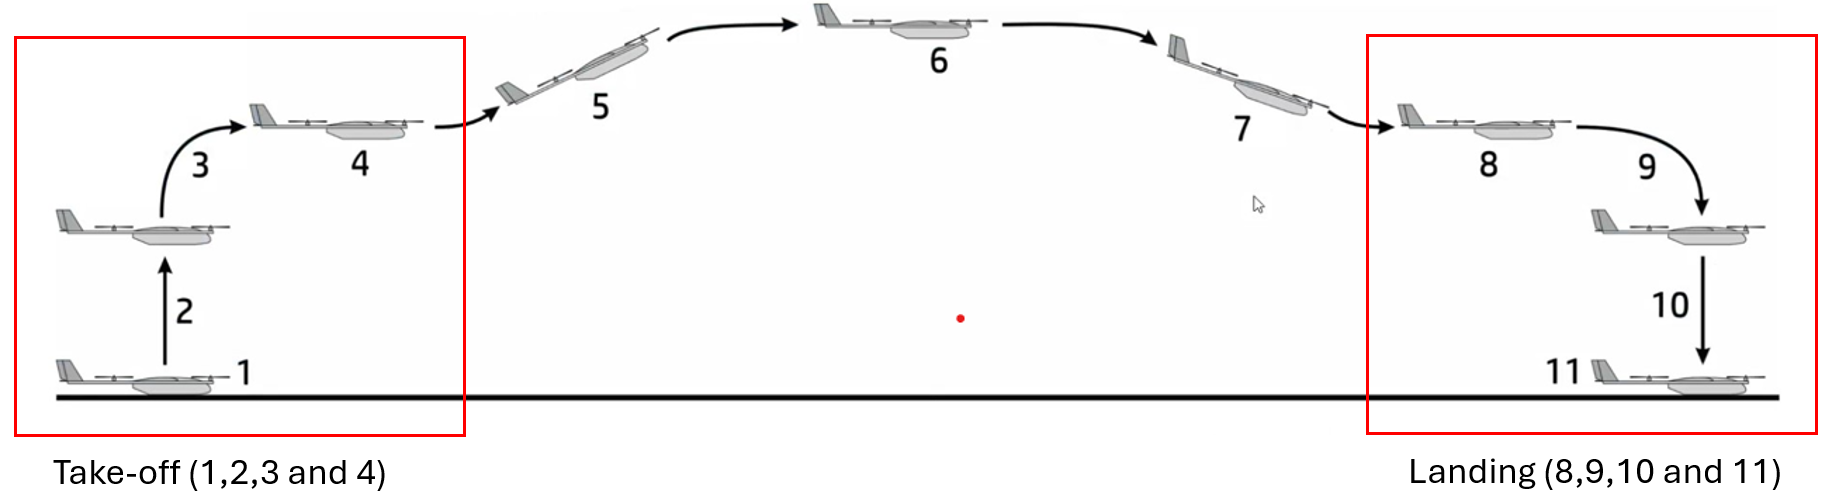
\includegraphics[width=\dimexpr\linewidth-11pt\relax]{images/passos.png}
      \caption{Ilustração das etapas de voo de um VTOL híbrido.}
      \label{fig:fases_voo}
\end{figure}

O objetivo principal é obter, a partir de dados de voo reais, um modelo matemático não-linear identificado que represente com fidelidade a dinâmica do modo quadricóptero. Esse modelo servirá como base para o desenvolvimento de algoritmos de controle e de um piloto automático (PA) para as manobras autônomas de decolagem e pouso vertical. A identificação é realizada a partir de curvas de empuxo e torque dos motores obtidas em bancada, dos momentos de inércia da aeronave e de dados coletados em manobras de voo específicas.

\section{Método M4V de Identificação}

Para a identificação do sistema, foi utilizada a metodologia M4V (Maneuver, Measurements, Methods, Models, Validation), uma abordagem estruturada e amplamente utilizada na identificação de sistemas de veículos aéreos [2]. A metodologia M4V divide o processo de identificação em fases bem definidas, garantindo uma abordagem sistemática e robusta.

\begin{figure}
      \centering
      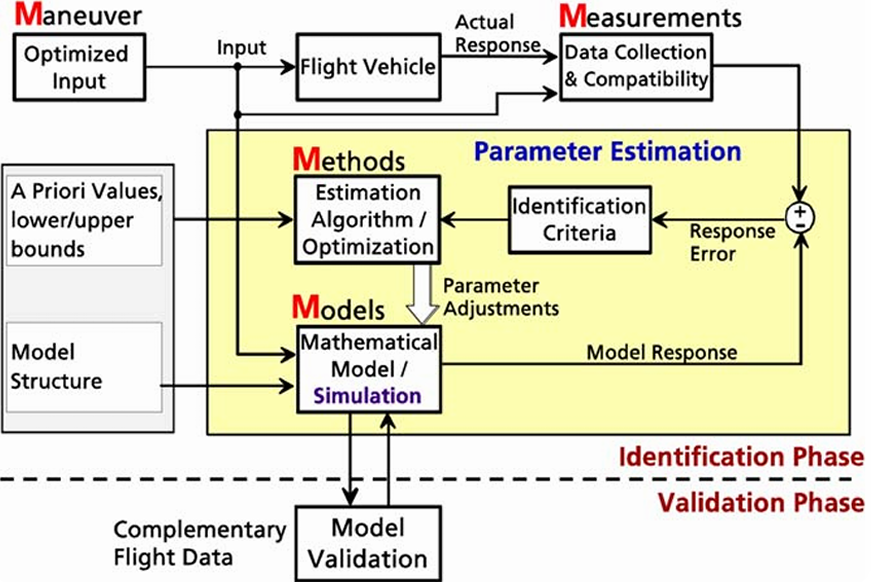
\includegraphics[width=\linewidth]{images/m4m.png}
      \caption{Diagrama do método M4V}
      \label{unet}
\end{figure}


\begin{RaggedRight}
As fases da metodologia M4V são:
\begin{itemize}
    \item \textbf{Maneuver (Manobra):} Entradas otimizadas são projetadas e aplicadas ao veículo em voo para excitar adequadamente a sua dinâmica.
    \item \textbf{Measurements (Medições):} Os dados da resposta real da aeronave às manobras são coletados por meio de sensores embarcados. A compatibilidade e a qualidade dos dados são verificadas nesta fase.
    \item \textbf{Methods (Métodos):} Algoritmos de estimação e otimização são utilizados para identificar os parâmetros do modelo matemático. O ajuste é feito com base em critérios de identificação, em particular na minimização do erro entre resposta real e simulada.
    \item \textbf{Models (Modelos):} Um modelo matemático estrutural, com valores iniciais (a priori), é continuamente refinado com os parâmetros estimados até que o erro seja minimizado.
\end{itemize}
\end{RaggedRight}

Após a fase de identificação, o modelo obtido é submetido a uma fase de validação, na qual dados de voo complementares, não utilizados na estimação, são usados para verificar a capacidade preditiva e a robustez do modelo.

\section{Modelo Matemático do Modo Quadricóptero}

O modelo matemático foi desenvolvido considerando a aeronave como um corpo rígido operando no modo quadricóptero. Neste modo, a sustentação e o controle de atitude são realizados exclusivamente pelos quatro motores verticais, enquanto o motor traseiro de cruzeiro e as superfícies aerodinâmicas permanecem inativos. Embora a configuração VTOL híbrida introduza particularidades na distribuição de massa e na geometria da aeronave em relação a um quadricóptero convencional, a dinâmica neste modo é governada unicamente pelas forças e momentos gerados pelos rotores verticais. As Figuras~\ref{fig:drone_config} e~\ref{fig:drone_real} ilustram a disposição dos motores, com os momentos e as forças por eles aplicados, e a aeronave real.

\begin{figure}
      \centering
      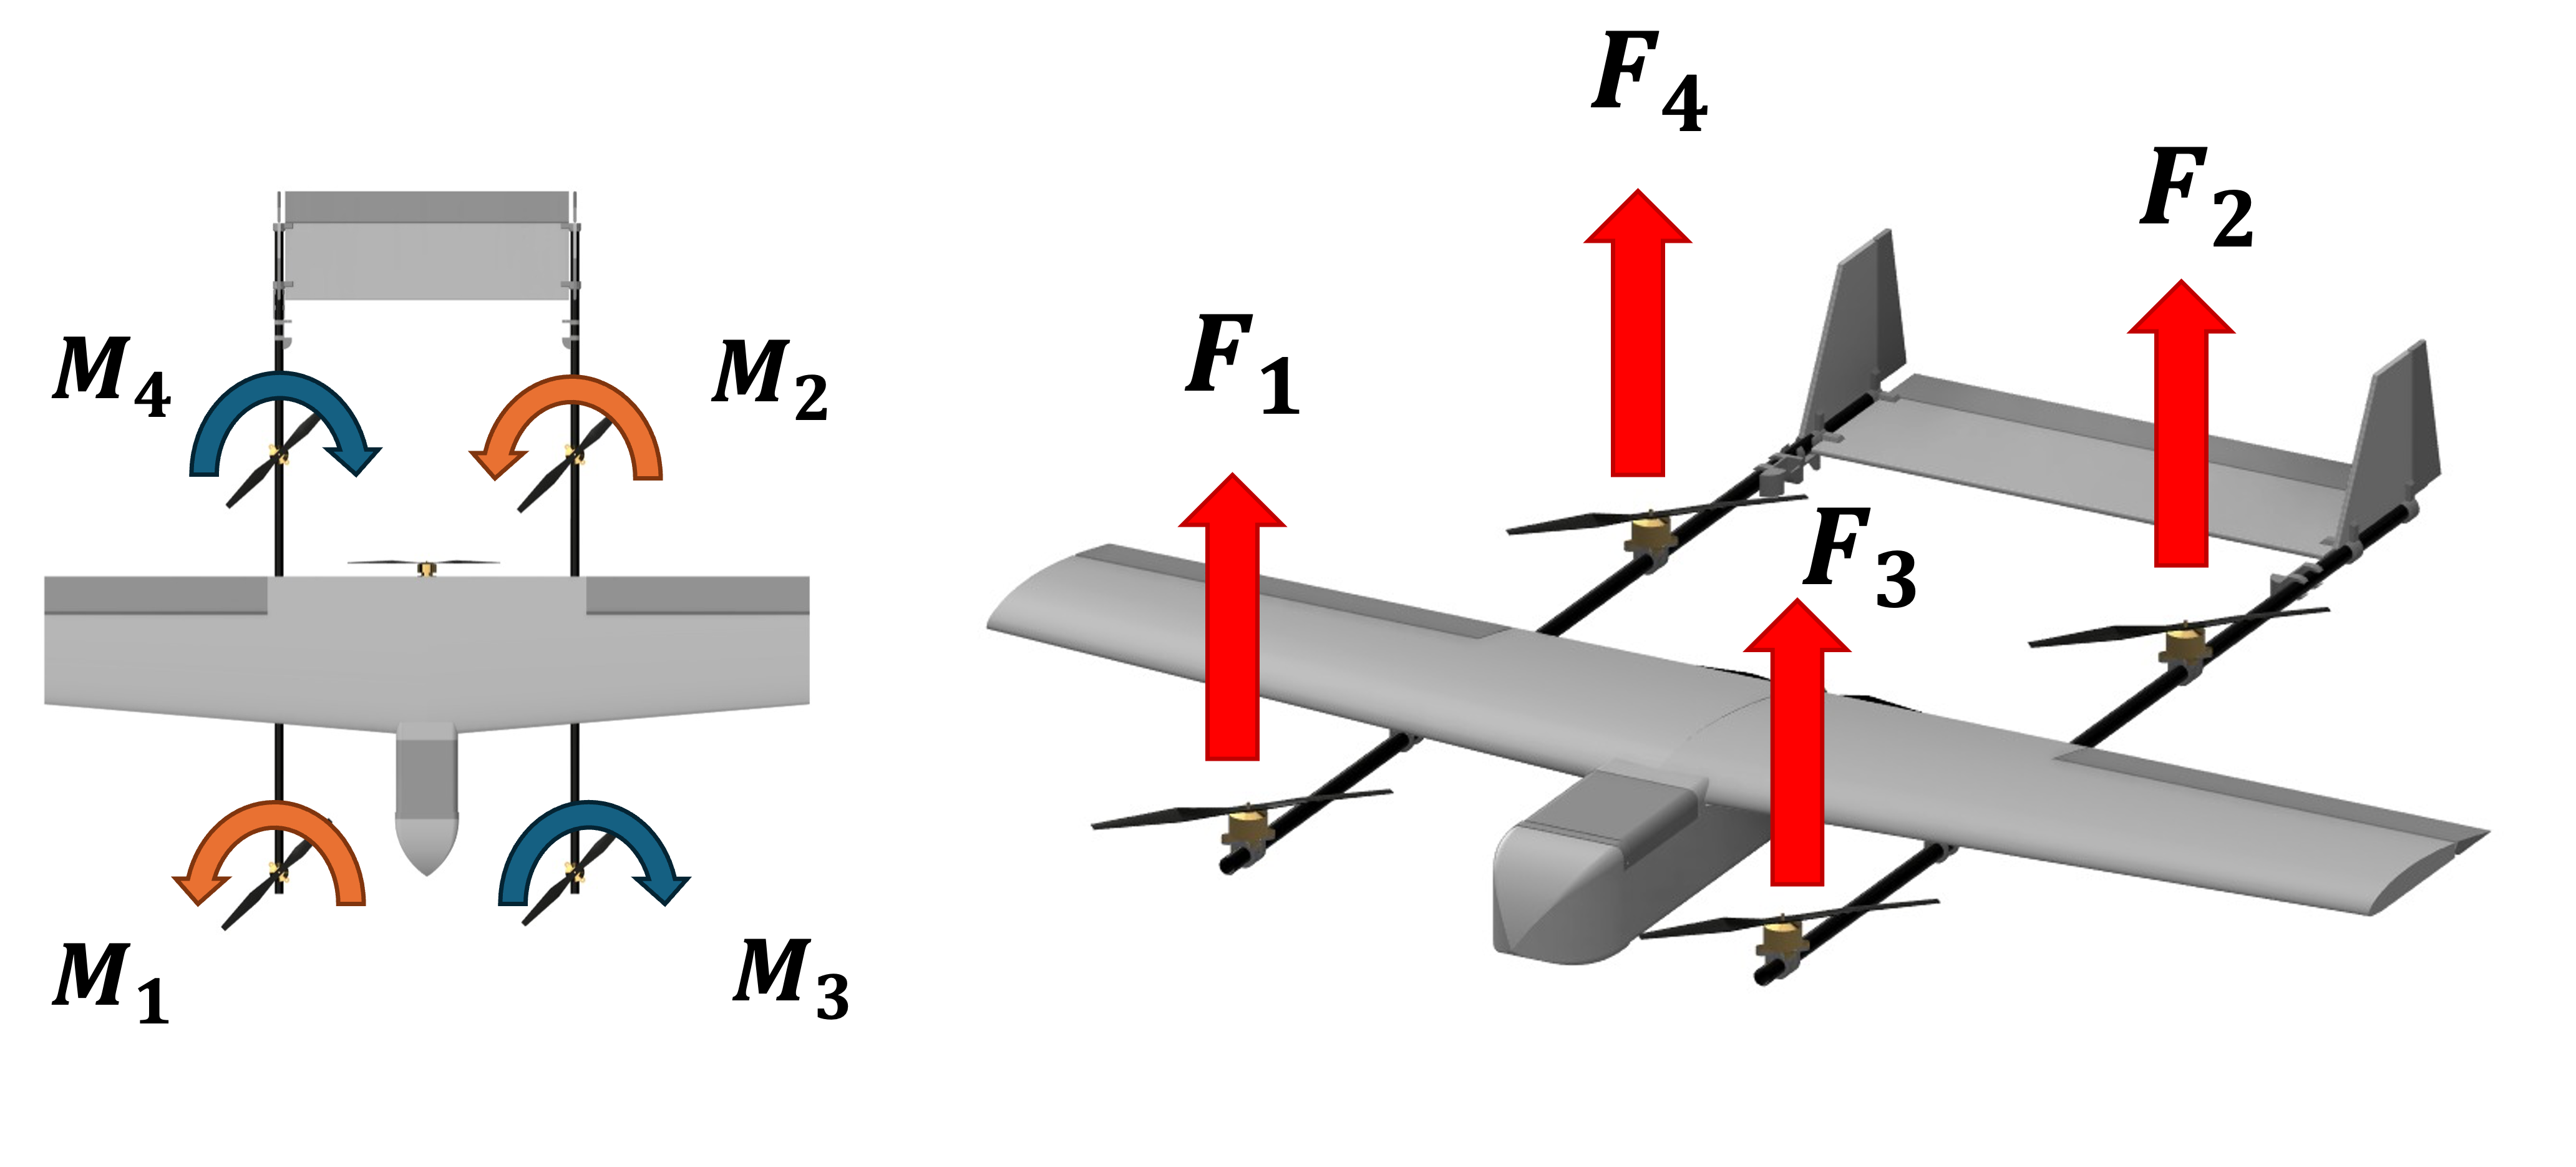
\includegraphics[width=\linewidth]{images/forcas-momentos.png}
      \caption{Relação de momentos e forças aplicados pelos motores.}
      \label{fig:drone_config}
\end{figure}

\begin{figure}
      \centering
      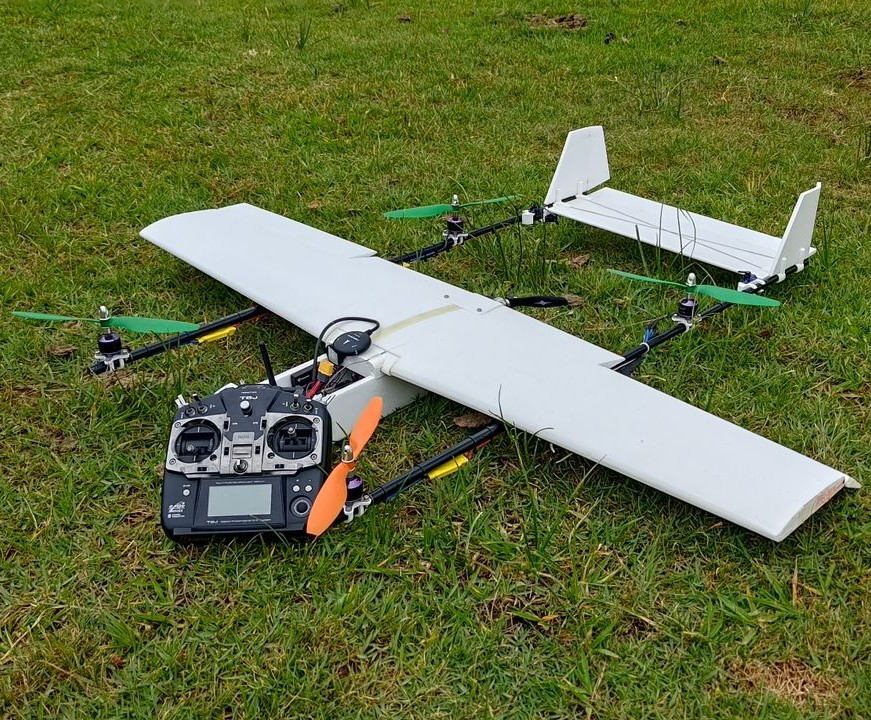
\includegraphics[width=\dimexpr\linewidth-11pt\relax]{images/rdrone.jpeg}
      \caption{Aeronave DH Hybrid-Drone VTOL.}
      \label{fig:drone_real}
\end{figure}

O modelo é descrito por um conjunto de equações de estado não-lineares. Os vetores de estado ($x$) e de entrada ($u$) são definidos como:
\begin{equation}
x = [\phi, \theta, \psi, p, q, r, u, v, w]^T
\end{equation}
\begin{equation}
u = [\sigma_1, \sigma_2, \sigma_3, \sigma_4]^T
\end{equation}
Onde $\phi, \theta, \psi$ são os ângulos de Euler (rolagem, arfagem e guinada); $p, q, r$ são as velocidades angulares no referencial do corpo; $u, v, w$ são as velocidades lineares no sistema de eixos do corpo; e $\sigma_i$ são os comandos de PWM normalizados enviados aos quatro motores do multirotor [3], detalhados a seguir no modelo do motor.

\subsection{Modelo do Motor}

O modelo do motor descreve a cadeia que converte o comando de PWM de cada motor nos esforços generalizados aplicados ao corpo rígido: o comando normalizado $\sigma_i$ é convertido em velocidade angular do rotor $\Omega_i$, que produz o empuxo $T_i$ e o contra-torque $Q_i$; esses esforços individuais são, por fim, combinados pela matriz de alocação no empuxo total $T$ e nos momentos $\tau_x$, $\tau_y$ e $\tau_z$ [13]. A Figura~\ref{fig:blocos_motor} apresenta a estrutura em dois estágios desse modelo, e cada etapa da cadeia foi caracterizada por meio de ensaios estáticos em bancada dinamométrica, nos quais foram medidos, para diferentes níveis de comando, a velocidade angular, o empuxo e o contra-torque do motor.

\begin{figure}[htbp]
      \centering
      
\includegraphics[width=\linewidth]{images/blocos-motor.png}
      \caption{Diagrama de blocos do modelo do motor: o ESC converte o comando normalizado $\sigma_i$ em velocidade angular de regime permanente (Equação~\eqref{eq:omega-ss}), filtrada pela dinâmica de primeira ordem (Equação~\eqref{eq:omega-lag}) e transformada em empuxo e contra-torque (Equação~\eqref{eq:tq}). Adaptado de [13].}
      \label{fig:blocos_motor}
\end{figure}

O comando de cada motor é a largura de pulso $\delta_{PWM,i}$, normalizada para o intervalo $[0,1]$:
\begin{equation}
\sigma_i = \frac{\delta_{PWM,i} - \delta_{\min}}{\delta_{\max} - \delta_{\min}}
\label{eq:norm}
\end{equation}
em que $\delta_{\min} = 1000~\mu$s e $\delta_{\max} = 2000~\mu$s são os limites da faixa de operação do ESC.

A primeira etapa da cadeia relaciona o comando normalizado com a velocidade angular do rotor. Em regime permanente, os dados de bancada da Figura~\ref{fig:motor_pwm_rpm} mostram que essa relação é bem aproximada por uma reta [13]:
\begin{equation}
\Omega_{ss,i} = C_R\,\sigma_i + \Omega_b
\label{eq:omega-ss}
\end{equation}
onde $C_R$ é o ganho do conjunto ESC--motor e $\Omega_b$ é a velocidade angular mínima de operação. O ajuste por mínimos quadrados aos pontos medidos, excluindo o ponto de motor parado, resulta em $C_R = 4523$~RPM e $\Omega_b = 1837$~RPM.

\begin{figure}[htbp]
      \centering
      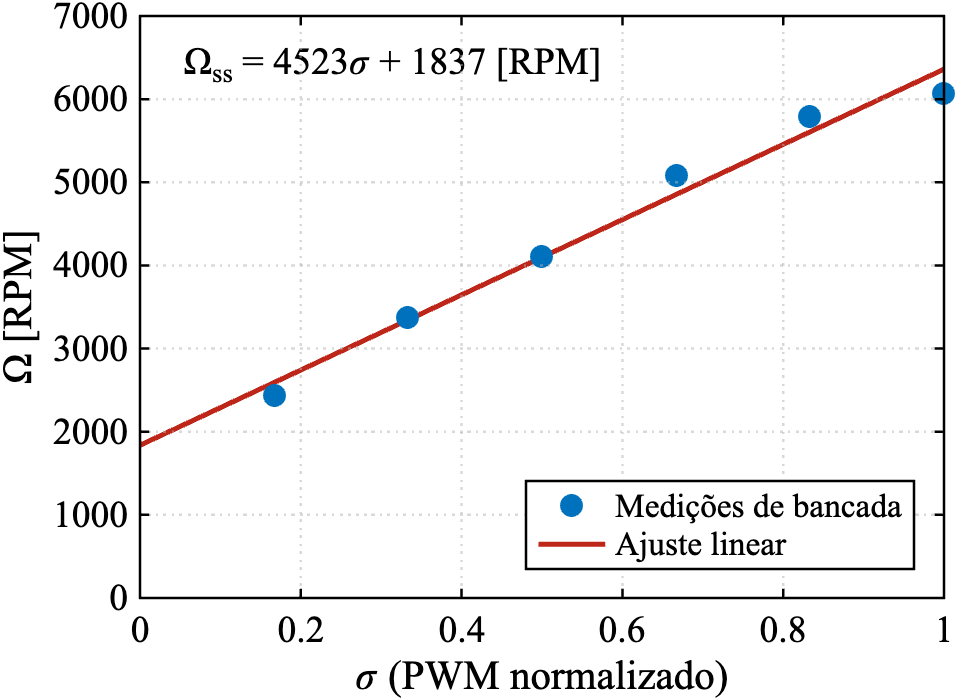
\includegraphics[width=0.9\linewidth]{images/motor_pwm_rpm.png}
      \caption{Velocidade angular do rotor em regime permanente em função do comando PWM normalizado. Os pontos são as medições de bancada e a linha contínua é o ajuste linear da Equação~\eqref{eq:omega-ss}.}
      \label{fig:motor_pwm_rpm}
\end{figure}

A resposta do conjunto ESC--motor--hélice não é instantânea: a velocidade angular converge para o valor de regime com uma dinâmica bem aproximada por um sistema de primeira ordem que, no domínio da frequência, corresponde a um filtro passa-baixas [13]:
\begin{equation}
\Omega_i(s) = \frac{1}{\tau_m s + 1}\,\Omega_{ss,i}(s)
\label{eq:omega-lag}
\end{equation}
em que $s$ é a variável de Laplace e $\tau_m = 0{,}05$~s é a constante de tempo adotada. A velocidade angular instantânea $\Omega_i$ resultante dessa dinâmica é a grandeza que efetivamente gera os esforços do rotor.

Cada rotor, girando com velocidade $\Omega_i$, produz um empuxo e um contra-torque proporcionais ao quadrado dessa velocidade [11], [13]:
\begin{equation}
T_i = c_{T_i}\,\Omega_i^{2}, \qquad Q_i = c_{M_i}\,\Omega_i^{2}
\label{eq:tq}
\end{equation}
onde $c_{T_i}$ e $c_{M_i}$ são os coeficientes de empuxo e de torque, dependentes da geometria da hélice e da densidade do ar, tratados como parâmetros identificáveis do modelo. O ajuste quadrático aos dados de bancada, apresentado na Figura~\ref{fig:motor_tq}, fornece os valores de referência $c_T = 1{,}76\times10^{-7}$~N/RPM$^2$ e $c_M = 5{,}04\times10^{-9}$~N$\cdot$m/RPM$^2$, adotados como valores iniciais do processo de identificação (Tabela~\ref{tab:const_iniciais}), no qual são refinados individualmente para cada motor.

\begin{figure}[htbp]
      \centering
      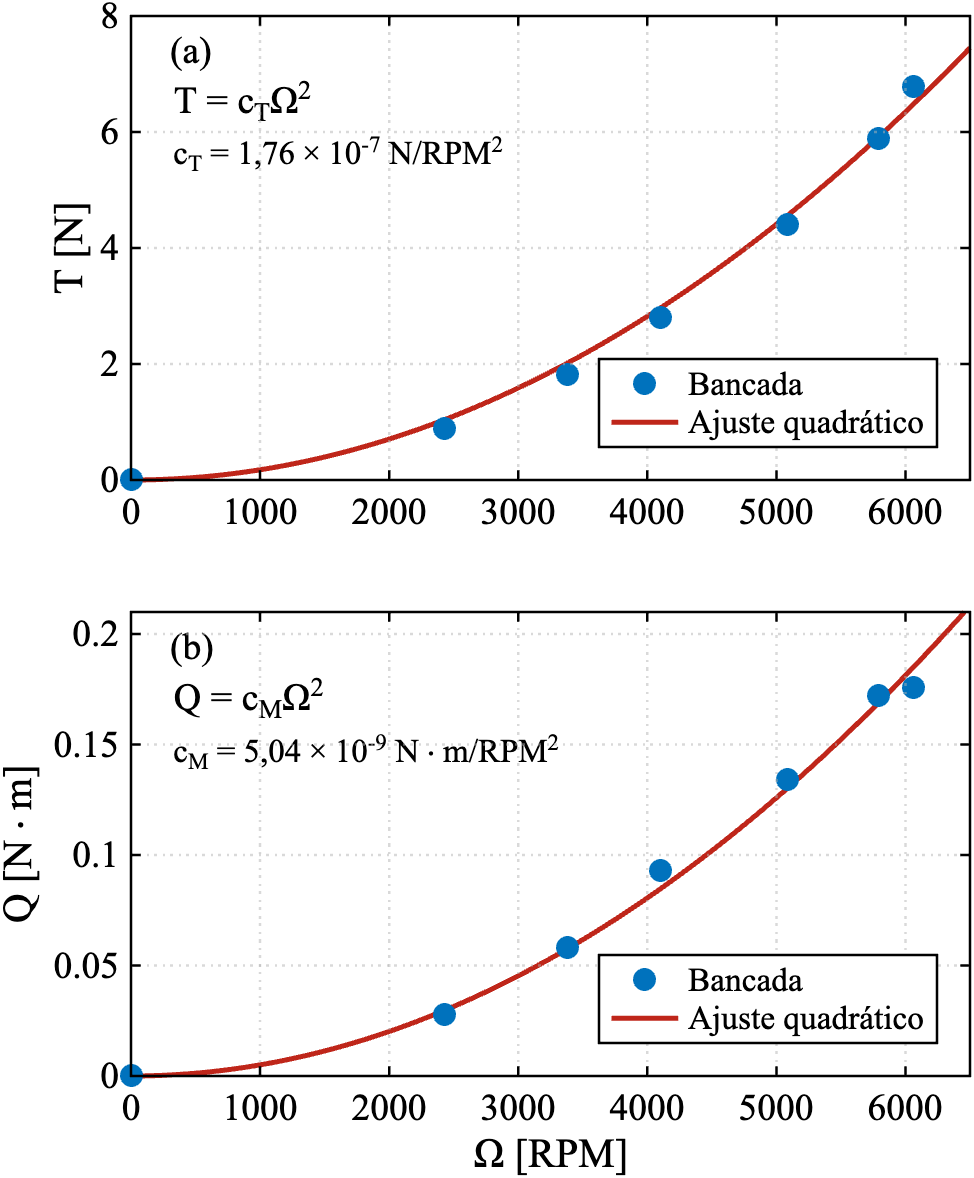
\includegraphics[width=\linewidth]{images/motor_thrust_torque.png}
      \caption{Empuxo (a) e contra-torque (b) em função da velocidade angular do rotor. Os pontos são as medições de bancada e as linhas contínuas são os ajustes quadráticos da Equação~\eqref{eq:tq}.}
      \label{fig:motor_tq}
\end{figure}

Os esforços individuais combinam-se em função da geometria da aeronave. Os momentos de rolagem e arfagem resultam do empuxo diferencial dos motores, ponderado pelas distâncias de cada rotor ao centro de gravidade: $L_{x_r}$ e $L_{x_l}$ são os braços laterais dos rotores dos lados direito (motores 1 e 4) e esquerdo (motores 2 e 3), e $L_{y_f}$ e $L_{y_r}$ são os braços longitudinais dos rotores dianteiros (motores 1 e 3) e traseiros (motores 2 e 4), distintos entre si na configuração H-frame. O momento de guinada, por sua vez, é gerado pelo contra-torque das hélices: os motores 1 e 2 giram em um sentido e os motores 3 e 4 no sentido oposto, de modo a cancelar o torque resultante em voo pairado [5]. Da Equação~\eqref{eq:tq} obtém-se a relação entre o contra-torque e o empuxo de cada rotor:
\begin{equation}
Q_i = \frac{c_M}{c_T}\,T_i
\label{eq:qt-ratio}
\end{equation}
que permite expressar os contra-torques em função dos empuxos, reunindo todas as contribuições em uma única matriz de alocação $\mathbf{B}$:
\begin{equation}
\begin{bmatrix} T \\ \tau_x \\ \tau_y \\ \tau_z \end{bmatrix}
=
\underbrace{\begin{bmatrix}
1 & 1 & 1 & 1 \\
-L_{x_r} & L_{x_l} & L_{x_l} & -L_{x_r} \\
L_{y_f} & -L_{y_r} & L_{y_f} & -L_{y_r} \\
\tfrac{c_M}{c_T} & \tfrac{c_M}{c_T} & -\tfrac{c_M}{c_T} & -\tfrac{c_M}{c_T}
\end{bmatrix}}_{\mathbf{B}}
\begin{bmatrix} T_1 \\ T_2 \\ T_3 \\ T_4 \end{bmatrix}
\label{eq:aloca}
\end{equation}

O modelo do motor estabelece, assim, o caminho completo das medidas de bancada ao modelo dinâmico: dos pares PWM--velocidade angular obtém-se $C_R$; dos pares velocidade angular--empuxo e velocidade angular--contra-torque obtêm-se $c_T$ e $c_M$, que geram os empuxos $T_1$ a $T_4$; e a matriz de alocação converte esses empuxos no empuxo total $T$, que alimenta o modelo translacional, e nos momentos $\tau_x$, $\tau_y$ e $\tau_z$, que alimentam o modelo rotacional.

\subsection{Modelo Translacional}

No modo quadricóptero, a única força propulsiva é o empuxo total $T$, que atua na direção negativa do eixo $z$ do corpo, $F = [0,\, 0,\, -T]^T$ [4]. Somando a projeção da gravidade no referencial do corpo e considerando que, em torno do voo pairado, as velocidades de translação são reduzidas, o que permite desprezar a sustentação e o arrasto aerodinâmico da estrutura de asa fixa, as equações de aceleração translacional são dadas por:

\begin{align}
\dot{u} &= rv - qw - g\sin\theta \\
\dot{v} &= pw - ru + g\sin\phi\cos\theta \\
\dot{w} &= qu - pv + g\cos\phi\cos\theta - \frac{T}{m}
\end{align}

Onde $T$ é o empuxo total obtido da matriz de alocação (Equação~\eqref{eq:aloca}), $g$ é a aceleração da gravidade e $m$ é a massa total da aeronave.

\subsection{Modelo Rotacional}

A dinâmica rotacional do corpo rígido é governada pelo tensor de inércia $\mathbf{J}$, que relaciona as velocidades angulares com os momentos angulares da aeronave. Para o referencial do corpo com origem no centro de gravidade, o tensor de inércia é dado por:
\begin{align}
\mathbf{J} = \begin{bmatrix}
J_{xx} & 0 & -J_{xz} \\
0 & J_{yy} & 0 \\
-J_{xz} & 0 & J_{zz}
\end{bmatrix}
\end{align}
onde $J_{xx}$, $J_{yy}$ e $J_{zz}$ são os momentos de inércia em torno dos eixos $x$, $y$ e $z$ do corpo, respectivamente, e $J_{xz}$ é o produto de inércia cruzado. Os produtos $J_{xy}$ e $J_{yz}$ são nulos por simetria do plano $xz$. No entanto, o produto de inércia $J_{xz}$ é não-nulo, uma vez que a aeronave possui configuração H-frame com braços dianteiros e traseiros de comprimentos distintos, o que resulta em uma distribuição de massa assimétrica em relação ao plano $xy$. Essa assimetria introduz acoplamento entre os eixos de rolagem e guinada, tornando o produto $J_{xz}$ um parâmetro relevante na modelagem e identificação do sistema.

As equações de momento do corpo rígido utilizam constantes $\Gamma_i$ derivadas dos momentos e produtos de inércia da aeronave. Definindo $\Gamma_0 = J_{xx} J_{zz} - J_{xz}^2$, as constantes são:

\begin{align}
\Gamma_1 &= \frac{J_{xz}(J_{xx} - J_{yy} + J_{zz})}{\Gamma_0} \\
\Gamma_2 &= \frac{J_{zz}(J_{zz} - J_{yy}) + J_{xz}^2}{\Gamma_0} \\
\Gamma_3 &= \frac{J_{zz}}{\Gamma_0} \quad , \quad
\Gamma_4 = \frac{J_{xz}}{\Gamma_0} \\
\Gamma_5 &= \frac{J_{zz} - J_{xx}}{J_{yy}} \quad , \quad
\Gamma_6 = \frac{J_{xz}}{J_{yy}} \\
\Gamma_7 &= \frac{J_{xx}(J_{xx} - J_{yy}) + J_{xz}^2}{\Gamma_0} \\
\Gamma_8 &= \frac{J_{xx}}{\Gamma_0}
\end{align}

As equações de momento são então dadas por:
\begin{align}
\dot{p} &= \Gamma_1 pq - \Gamma_2 qr + \Gamma_3 \tau_x + \Gamma_4 \tau_z - c_p\, p \\
\dot{q} &= \Gamma_5 pr - \Gamma_6 (p^2 - r^2) + \frac{1}{J_{yy}}\tau_y - c_q\, q \\
\dot{r} &= \Gamma_7 pq - \Gamma_1 qr + \Gamma_4 \tau_x + \Gamma_8 \tau_z - c_r\, r
\end{align}

Onde $\tau_x, \tau_y, \tau_z$ são os momentos de controle gerados pelos motores, obtidos da matriz de alocação (Equação~\eqref{eq:aloca}). Os termos $c_p$, $c_q$ e $c_r$ são coeficientes de amortecimento angular, que modelam a dissipação de energia rotacional devido ao arrasto aerodinâmico das hélices e da fuselagem [13]. Esses coeficientes são proporcionais à velocidade angular no respectivo eixo, de modo que quanto maior a velocidade de rotação, maior o momento de amortecimento que se opõe ao movimento, e são parâmetros a serem estimados no processo de identificação, juntamente com os momentos de inércia e os coeficientes dos motores.

As equações da cinemática dos ângulos de Euler são:

\begin{align}
\dot{\phi} &= p + \tan\theta(q\sin\phi + r\cos\phi) \\
\dot{\theta} &= q\cos\phi - r\sin\phi \\
\dot{\psi} &= \frac{q\sin\phi + r\cos\phi}{\cos\theta}
\end{align}

\section{Estimação de Parâmetros}

A estimação dos parâmetros do modelo do modo quadricóptero combina dois métodos complementares no domínio do tempo: o Método de Erro de Equação (\textit{Equation Error Method} -- EEM), que fornece uma estimativa inicial algébrica, e o Método de Erro de Saída (\textit{Output Error Method} -- OEM), que a refina por máxima verossimilhança [2]. Ambos buscam o vetor de parâmetros $\Theta$ que minimiza os resíduos entre as saídas medidas $z$ e as simuladas pelo modelo $y(\Theta)$.

O modelo da seção anterior é escrito na forma de espaço de estados $\dot{x} = f(x, u, \Theta)$, em que o vetor de parâmetros a identificar reúne os momentos e o produto de inércia, os coeficientes de empuxo e de contra-torque de cada motor (Equação~\eqref{eq:tq}) e os coeficientes de amortecimento rotacional:
\begin{equation}
\Theta = [\,J_{xx},\,J_{yy},\,J_{zz},\,J_{xz},\;c_{T_1},\dots,c_{T_4},\;c_{M_1},\dots,c_{M_4},\;c_p,\,c_q,\,c_r\,]^{\top}
\label{eq:theta}
\end{equation}
Os coeficientes $c_{T_i}$ e $c_{M_i}$ partem dos valores de bancada e são refinados individualmente para cada motor, enquanto $J_{zz}$ e $J_{xz}$ são mantidos fixos nos valores de projeto (CAD), por serem pouco observáveis dada a baixa autoridade de controle do eixo de guinada. A identificação concentra-se no subsistema rotacional: como as equações de momento do modelo rotacional são autônomas nas velocidades angulares, basta integrar esse subsistema, alimentado pelos momentos reconstruídos dos comandos PWM pelo modelo do motor e pela matriz de alocação (Equação~\eqref{eq:aloca}), comparando às medições as taxas simuladas e as forças específicas do acelerômetro.

\subsection{Método de Erro de Equação (EEM)}

O EEM dispensa a integração numérica do modelo: a equação dinâmica é avaliada diretamente sobre os estados medidos e suas derivadas. O resíduo de equação é definido como a diferença entre a derivada angular medida e a prevista pelas equações de momento do modelo rotacional:
\begin{equation}
e_{\text{EEM}}(t_k) = \dot{\omega}_{\text{med}}(t_k) - f_\omega\big(\omega_{\text{med}}(t_k),\, \tau(t_k),\, \Theta\big)
\label{eq:eem-res}
\end{equation}
com $\omega = [p, q, r]^{\top}$. Os parâmetros são obtidos minimizando o erro quadrático ponderado sobre os segmentos de treino concatenados:
\begin{equation}
\Theta_{\text{EEM}} = \arg\min_{\Theta} \sum_{k} \big\| \mathbf{W}^{1/2}\, e_{\text{EEM}}(t_k) \big\|^2
\label{eq:eem-cost}
\end{equation}
em que $\mathbf{W} = \mathrm{diag}(1/\sigma_i^2)$ é a matriz diagonal de pesos que pondera cada canal pelo inverso da sua variância, e $\dot{\omega}_{\text{med}}$ é obtida por diferenciação numérica do sinal suavizado. Com as inércias fixadas nos valores iniciais, o resíduo da Equação~\eqref{eq:eem-res} é linear nos coeficientes dos motores e de amortecimento, tornando a Equação~\eqref{eq:eem-cost} um problema de mínimos quadrados de solução rápida e robusta. Em contrapartida, o uso das derivadas medidas, que amplificam o ruído, introduz viés, razão pela qual o EEM serve como ponto de partida, e não como estimativa final [2].

\subsection{Método de Erro de Saída (OEM)}

O OEM elimina esse viés ao comparar a saída \emph{integrada} do modelo com as medições. A partir de $\Theta_{\text{EEM}}$, o subsistema rotacional é integrado no tempo (Runge--Kutta de 4ª ordem) com a mesma entrada aplicada ao veículo, produzindo a saída simulada $y(t_k, \Theta)$; o resíduo é o erro de saída $z(t_k) - y(t_k, \Theta)$. As saídas reúnem as velocidades angulares $(p, q, r)$ e as forças específicas medidas pela IMU $(a_x, a_y, a_z)$, e a ponderação por $\mathbf{W}$ normaliza as diferentes grandezas (rad/s vs.\ m/s$^2$), evitando que os canais de maior magnitude dominem o ajuste.

Sob a hipótese de ruído de medição gaussiano com covariância $R$, o OEM é um estimador de máxima verossimilhança, que minimiza o custo [2]:
\begin{equation}
J(\Theta) = \frac{1}{2} \sum_{k=1}^{N} \big[z(t_k) - y(t_k,\Theta)\big]^{\top} R^{-1} \big[z(t_k) - y(t_k,\Theta)\big]
\label{eq:oem-cost}
\end{equation}
O mínimo é buscado pelo método de Gauss--Newton: linearizando a saída em torno da estimativa corrente, $y(\Theta + \delta) \approx y(\Theta) + S\,\delta$, com a matriz de sensibilidades
\begin{equation}
S(t_k) = \frac{\partial y(t_k, \Theta)}{\partial \Theta}
\label{eq:sens}
\end{equation}
o passo $\delta$ que anula o gradiente do custo resolve as equações normais
\begin{equation}
\Big[\textstyle\sum_{k} S_k^{\top} R^{-1} S_k\Big]\, \delta = \textstyle\sum_{k} S_k^{\top} R^{-1}\big[z(t_k) - y(t_k,\Theta)\big]
\label{eq:gauss-newton}
\end{equation}
cujo termo entre colchetes é a matriz de informação de Fisher $F$. Os parâmetros são então atualizados por:
\begin{equation}
\Theta_{j+1} = \Theta_{j} + \delta
\label{eq:update}
\end{equation}
O ciclo de integração do modelo para formar o erro de saída, e calcular as sensibilidades e atualizar os parâmetros, repete-se até a convergência, conforme ilustra a Figura~\ref{fig:opt_loop}. Na implementação, as sensibilidades são calculadas por diferenças finitas, a inversa da covariância $R^{-1}$ é aproximada pela matriz diagonal fixa de pesos $\mathbf{W} = \mathrm{diag}(1/\sigma_i^2)$, cujos elementos são o inverso da variância de cada canal de saída, e o passo $\delta$ é determinado pelo algoritmo \textit{Trust-Region Reflective}~[2] da função \texttt{lsqnonlin} do MATLAB, que globaliza o Gauss--Newton e impõe os limites físicos dos parâmetros.

\begin{figure}[htbp]
\centering
\begin{tikzpicture}[
    node distance=0.9cm,
    block/.style={rectangle, draw, rounded corners=2pt, minimum width=2.7cm, minimum height=0.7cm, align=center, font=\scriptsize},
    decis/.style={rectangle, draw, rounded corners=2pt, fill=orange!12, minimum width=2.4cm, minimum height=0.7cm, align=center, font=\scriptsize},
    arrow/.style={-{Stealth[length=2mm]}, semithick},
    dasharrow/.style={-{Stealth[length=2mm]}, semithick, dashed},
    lbl/.style={font=\tiny, fill=white, inner sep=1pt}
]

% --- Topo: Parâmetros (esquerda) e Medições (direita) ---
\node[block, fill=green!15] (theta)
    {$\Theta_j$ -- Par\^ametros atuais};

\node[block, fill=gray!15, right=1.5cm of theta] (data)
    {Medi\c{c}\~oes $z(t_k)$\\(sensores)};

% --- Coluna central (entre theta e data) ---
\node[block, fill=blue!10, below=0.9cm of $(theta.south)!0.5!(data.south)$] (model)
    {Modelo Matem\'atico\\(integra\c{c}\~ao RK4)};

\node[block, fill=blue!10, below=of model] (resid)
    {Erro de sa\'ida ponderado\\$\mathbf{W}^{1/2}\big[z(t_k) - y(t_k,\Theta)\big]$};

\node[block, fill=yellow!18, below=of resid] (lsq)
    {\textbf{Eq.~\eqref{eq:oem-cost}} -- $\min J(\Theta)$\\\texttt{lsqnonlin} (\textit{Trust-Region})};

\node[decis, below=of lsq] (conv) {Convergiu?};

\node[block, fill=red!10, below=of conv] (r2)
    {\textbf{Eq.~\eqref{eq:r2}} -- $R^2$ por canal\\(valida\c{c}\~ao)};

% --- Esquerda: interno lsqnonlin ---
\node[block, fill=yellow!18, left=0.5cm of lsq] (jac)
    {\textbf{Eq.~\eqref{eq:sens}} -- Sensibilidades\\$S = \partial y / \partial \Theta$};

\node[block, fill=green!15, left=0.5cm of resid] (update)
    {\textbf{Eq.~\eqref{eq:update}} -- Atualiza\c{c}\~ao\\$\Theta_{j+1} = \Theta_j + \delta$};

% === SETAS ===
\draw[arrow] (theta) |- (model);
\draw[arrow] (model) -- node[lbl, right] {$y(t_k,\Theta)$} (resid);
\draw[arrow] (resid) -- (lsq);
\draw[arrow] (lsq) -- (conv);
\draw[arrow] (conv) -- node[lbl, right] {Sim} (r2);

% Dados → resíduos (desce do topo)
\draw[arrow] (data) |- (resid);

% Interno lsqnonlin
\draw[dasharrow] (lsq) -- (jac);
\draw[dasharrow] (jac) -- (update);

% Não → atualização (contorna pelo lado esquerdo)
\coordinate (aux) at ([xshift=-0.7cm]jac.west);
\draw[arrow] (conv.west) -| node[lbl, near start, above] {N\~ao} (aux) |- (update.west);

% Loop de volta
\draw[arrow] (update) -- (theta);

% Caixa tracejada
\begin{scope}[on background layer]
\node[draw=gray, dashed, rounded corners=4pt, fill=gray!5,
      inner xsep=8pt, inner ysep=8pt,
      fit=(jac)(update),
      label={[font=\tiny, text=gray]above: }] {};
\end{scope}

\end{tikzpicture}
\caption{Ciclo iterativo do m\'etodo do erro de sa\'ida: o modelo \'e integrado com os par\^ametros correntes, o erro de sa\'ida alimenta o \texttt{lsqnonlin}, que calcula internamente as sensibilidades (Equa\c{c}\~ao~\eqref{eq:sens}) e o passo de atualiza\c{c}\~ao (Equa\c{c}\~ao~\eqref{eq:update}); ap\'os a converg\^encia, o ajuste \'e avaliado pelo $R^2$ (Equa\c{c}\~ao~\eqref{eq:r2}) no segmento de valida\c{c}\~ao. Adaptado de [2].}
\label{fig:opt_loop}
\end{figure}

A qualidade do ajuste é avaliada pelo coeficiente de determinação, calculado para cada canal de saída em um segmento de validação que não participa da otimização:
\begin{equation}
R^2 = 1 - \frac{\sum_{k}(z_k - y_k)^2}{\sum_{k}(z_k - \bar{z})^2}
\label{eq:r2}
\end{equation}
onde $\bar{z}$ é a média das medições, e valores próximos de 1 indicam boa aderência entre modelo e dados. Na convergência, a inversa da matriz de informação de Fisher $F$ (Equação~\eqref{eq:gauss-newton}) fornece a covariância das estimativas (limite de Cramér--Rao), de onde se extrai o desvio-padrão relativo de cada parâmetro; valores elevados sinalizam parâmetros pouco observáveis pelos dados [2].

\subsection{Método de Erro de Saída com Multijanelas}

Neste trabalho, a estimação dos parâmetros foi realizada por meio do Método de Erro de Saída (\textit{Output Error Method} -- OEM) com uma estratégia de multijanelas progressivas. Diferentemente do OEM convencional, que integra o modelo ao longo de todo o registro de voo com uma única condição inicial, a abordagem por multijanelas divide cada segmento de dados em janelas temporais menores. No início de cada janela, os estados do modelo são reinicializados com os valores medidos, de modo que os erros de integração não se propagam entre janelas adjacentes. Isso aumenta significativamente a robustez da identificação, pois impede que divergências locais contaminem o restante da simulação.

O processo de identificação é dividido em duas fases sequenciais, conforme ilustrado na Figura~\ref{fig:oem_diagram}:

\begin{itemize}
    \item \textbf{Fase A -- EEM (Equation Error Method):} Os dados de todos os segmentos de treino são concatenados e utilizados em uma formulação algébrica (sem integração numérica). Os parâmetros rotacionais são estimados minimizando o erro entre as derivadas angulares medidas e as calculadas pelo modelo. Esta fase fornece uma estimativa inicial robusta $\Theta_{\text{EEM}}$ para a Fase B.
    \item \textbf{Fase B -- OEM (Output Error Method) Progressivo:} Utilizando como valores iniciais de $\Theta$, os valores de $\Theta_{\text{EEM}}$, o modelo é integrado numericamente com RK4 dentro de cada janela. A duração das janelas é progressivamente aumentada ($T_w = 1\text{s} \to 2\text{s} \to 3\text{s}$), de modo que nas primeiras etapas o otimizador ajusta os parâmetros com menor risco de divergência, e nas etapas seguintes captura a dinâmica de mais longo prazo. A cada estágio, o desempenho é avaliado no segmento de validação, e o conjunto de parâmetros com melhor coeficiente de determinação $R^2$ é selecionado como resultado final $\Theta^*$.
\end{itemize}

A função de custo é a mesma do OEM (Equação~\eqref{eq:oem-cost}, com $R^{-1} \approx \mathbf{W}$), agora agregando os resíduos ponderados de todas as janelas de todos os segmentos de treino:
\begin{align}
J(\Theta) = \sum_{s=1}^{N_s} \sum_{w=1}^{N_w^{(s)}} \sum_{k \in \mathcal{W}_w^{(s)}} \left\| \mathbf{W}^{1/2} \left[ z(t_k) - y(t_k, \Theta) \right] \right\|^2
\end{align}
onde $N_s$ é o número de segmentos de treino, $N_w^{(s)}$ é o número de janelas no segmento $s$, $\mathcal{W}_w^{(s)}$ são os índices temporais da janela $w$, e $\mathbf{W}^{1/2}$ é a raiz quadrada da matriz de pesos conforme definido anteriormente. As saídas $z$ e $y$ incluem tanto as velocidades angulares $(p, q, r)$ quanto as forças específicas medidas pela IMU $(a_x, a_y, a_z)$.

\begin{figure}[htbp]
\centering
\resizebox{\linewidth}{!}{%
\begin{tikzpicture}[
    node distance=0.6cm and 0.4cm,
    block/.style={rectangle, draw, fill=blue!8, text width=2.2cm, minimum height=0.7cm, align=center, font=\scriptsize},
    bigblock/.style={rectangle, draw, fill=green!8, text width=2.8cm, minimum height=0.7cm, align=center, font=\scriptsize},
    smallblock/.style={rectangle, draw, fill=orange!10, text width=1.4cm, minimum height=0.55cm, align=center, font=\tiny},
    arrow/.style={-{Stealth[length=2mm]}, thick},
    every node/.style={font=\scriptsize}
]

% Top: Flight Data
\node[block, fill=gray!15, text width=3cm] (data) {Dados de Voo\\(PWM, $p,q,r$, $\phi,\theta,\psi$, IMU)};

% Segmentation
\node[block, below=0.5cm of data] (seg) {Segmenta\c{c}\~ao Temporal};

% Segments
\node[smallblock, below left=0.5cm and 0.6cm of seg] (s1) {Seg. 1};
\node[smallblock, below=0.5cm of seg] (s2) {Seg. 2};
\node[smallblock, below right=0.5cm and 0.6cm of seg] (sn) {Seg. $N_s$};
\node[smallblock, right=0.3cm of sn, fill=red!10] (val) {Valida\c{c}\~ao};

% Phase A
\node[bigblock, below=1.2cm of s2, fill=yellow!15, text width=4cm] (eembox) {\textbf{Fase A: EEM}\\Concatena segmentos\\Estima\c{c}\~ao alg\'ebrica $\to \Theta_{\text{EEM}}$};

% Initial parameters
\node[smallblock, left=0.9cm of eembox, fill=blue!10, text width=1.8cm] (theta0) {$\Theta_0$\\(valores iniciais)};

% Phase B
\node[bigblock, below=0.5cm of eembox, fill=green!12, text width=4cm] (oembox) {\textbf{Fase B: OEM Progressivo}};

% Windows inside OEM
\node[smallblock, below left=0.5cm and 0.4cm of oembox, fill=green!20, text width=1.8cm] (w1) {$T_w=1$s\\$\Rightarrow \Theta_{\text{OEM},1}$};
\node[smallblock, below=0.5cm of oembox, fill=green!20, text width=1.8cm] (w2) {$T_w=2$s\\$\Rightarrow \Theta_{\text{OEM},2}$};
\node[smallblock, below right=0.5cm and 0.4cm of oembox, fill=green!20, text width=1.8cm] (w3) {$T_w=3$s\\$\Rightarrow \Theta_{\text{OEM},3}$};

% Best selection
\node[block, below=1.2cm of w2, fill=red!10, text width=3.2cm] (best) {Seleciona melhor $R^2$\\no segmento de valida\c{c}\~ao\\$\Theta^*$};

% Arrows
\draw[arrow] (data) -- (seg);
\draw[arrow] (seg) -- (s1);
\draw[arrow] (seg) -- (s2);
\draw[arrow] (seg) -- (sn);
\draw[arrow] (seg) -- (val);

\draw[arrow] (s1) -- (eembox);
\draw[arrow] (s2) -- (eembox);
\draw[arrow] (sn) -- (eembox);

\draw[arrow] (theta0) -- (eembox);

\draw[arrow] (eembox) -- node[right, font=\tiny] {$\Theta_{\text{EEM}}$} (oembox);

\draw[arrow] (oembox) -- (w1);
\draw[arrow] (oembox) -- (w2);
\draw[arrow] (oembox) -- (w3);

\draw[arrow] (w1) -- (best);
\draw[arrow] (w2) -- (best);
\draw[arrow] (w3) -- (best);

% Validation arrow
\draw[arrow, dashed] (val.south) |- (best.east);

\end{tikzpicture}%
}
\caption{Diagrama do processo de identifica\c{c}\~ao por OEM com multijanelas progressivas. A partir dos valores iniciais $\Theta_0$, a Fase~A (EEM alg\'ebrico) fornece $\Theta_{\text{EEM}}$, que inicializa a Fase~B (OEM com janelas de dura\c{c}\~ao crescente); cada janela gera um modelo $\Theta_{\text{OEM},i}$, e o melhor conjunto de par\^ametros $\Theta^*$ \'e selecionado com base no $R^2$ do segmento de valida\c{c}\~ao.}
\label{fig:oem_diagram}
\end{figure}

A reinicialização dos estados no início de cada janela é um aspecto fundamental da abordagem. Dentro de cada janela $w$, o integrador RK4 parte das condições iniciais medidas $z(t_{w,0})$ e propaga os estados até o final da janela. Essa técnica, conhecida como \textit{multiple shooting}, garante que o erro de cada janela dependa apenas da qualidade local dos parâmetros, e não do acúmulo de erros de janelas anteriores.

\section{Metodologia}

A abordagem metodológica deste trabalho é fundamentada na estrutura de identificação de sistemas M4V. As etapas práticas envolveram a coleta de dados de voo no modo quadricóptero por meio de manobras específicas, a determinação de constantes iniciais para o modelo e a implementação do modelo matemático em ambiente de simulação para o processo de identificação.

\subsection{Manobras e Dados para Identificação}

A qualidade da identificação depende diretamente da riqueza dos dados coletados. Para garantir excitação suficiente da dinâmica do modo quadricóptero, foram executadas manobras de voo projetadas para excitar os modos de movimento em torno dos eixos principais: rolagem, arfagem e guinada [7] [8]. Todas as manobras foram realizadas com a aeronave operando exclusivamente no modo quadricóptero, com o motor de cruzeiro desligado.

Os dados foram extraídos diretamente dos logs de voo da aeronave [9] e divididos em dois conjuntos:

\begin{sloppypar}
\begin{itemize}
    \item \textbf{Entradas do Sistema ($u$):} Sinais de Modulação por Largura de Pulso (PWM) enviados aos quatro motores verticais, registrados ao longo do tempo durante as manobras.
    \item \textbf{Saídas do Sistema ($y$):} Velocidades angulares nos eixos do corpo -- rolagem ($p$), arfagem ($q$) e guinada ($r$) -- e forças específicas medidas pela IMU ($a_x$, $a_y$, $a_z$), em radianos por segundo e m/s$^2$, respectivamente.
\end{itemize}
\end{sloppypar}

\begin{figure}
      \centering
      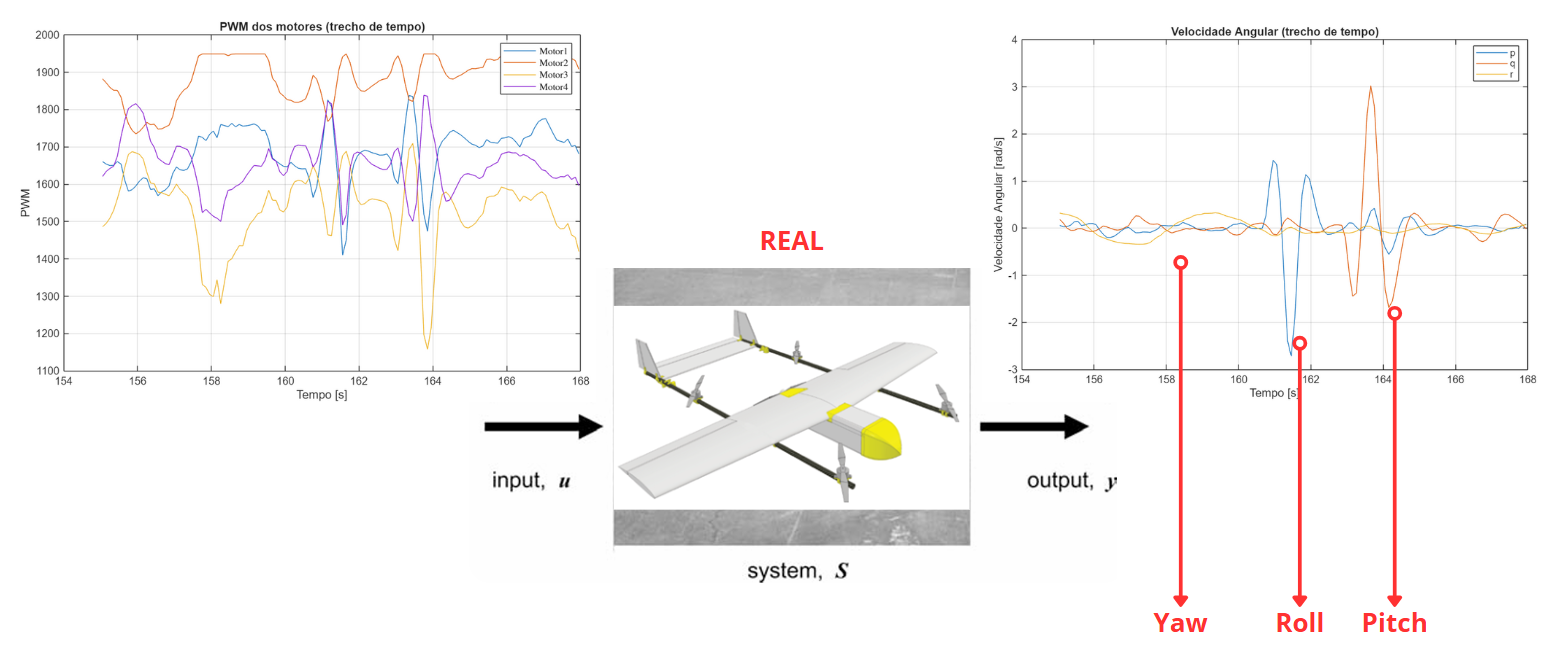
\includegraphics[width=\linewidth]{images/measurements.png}
      \caption{Dados de Identificação}
\end{figure}

\subsection{Constantes Iniciais}
\begin{sloppypar}
As constantes iniciais do modelo foram obtidas por meio de medições físicas da aeronave e dos ensaios em bancada do modelo do motor. As distâncias entre cada rotor e o centro de gravidade, que definem os braços de momento da matriz de alocação, são apresentadas na Figura~\ref{fig:bracos}, e os principais valores iniciais são reunidos na Tabela~\ref{tab:const_iniciais}.
\end{sloppypar}

\begin{figure}[htbp]
      \centering
      
\includegraphics[width=0.8\linewidth]{images/bracos.png}
      \caption{Distâncias entre os motores e o CG.}
      \label{fig:bracos}
\end{figure}

\begin{table}[htbp]
\centering
\begin{tabular}{l|c|c|l}
\hline
\textbf{Parâmetro} & \textbf{Valor} & \textbf{Unidade} & \textbf{Modo de obtenção} \\
\hline
$L_{x_l} = L_{x_r}$ & 0,232 & m & Medição física \\
$L_{y_f}$ & 0,330 & m & Medição física \\
$L_{y_r}$ & 0,323 & m & Medição física \\
$c_T$ & $1{,}76\times10^{-7}$ & N/RPM$^2$ & Ensaio em bancada \\
$c_M$ & $5{,}04\times10^{-9}$ & N$\cdot$m/RPM$^2$ & Ensaio em bancada \\
$m$ & 1,993 & kg & Medição física com balança \\
\hline
\end{tabular}
\caption{Valores iniciais do modelo.}
\label{tab:const_iniciais}
\end{table}

Substituindo na Equação~\eqref{eq:aloca} as distâncias medidas e a razão entre os coeficientes de bancada $c_M/c_T = 0{,}0286$~m, a matriz de alocação assume a forma numérica:
\begin{equation}
\mathbf{B}=
\begin{bmatrix}
1 & 1 & 1 & 1 \\
-0{,}232 & 0{,}232 & 0{,}232 & -0{,}232 \\
0{,}330 & -0{,}323 & 0{,}330 & -0{,}323 \\
0{,}0286 & 0{,}0286 & -0{,}0286 & -0{,}0286
\end{bmatrix}
\label{eq:aloca_num}
\end{equation}
A última linha, associada à guinada, é cerca de uma ordem de grandeza menor que as de rolagem e arfagem, o que antecipa a menor autoridade de controle e a menor observabilidade desse eixo na identificação.

Também foi medido o desalinhamento da IMU em relação ao centro de gravidade, apresentado na Figura~\ref{fig:imu_offset}, necessário para relacionar as forças específicas registradas pelo sensor com a dinâmica do centro de gravidade.

\begin{figure}[htbp]
      \centering
      
\includegraphics[width=\linewidth]{images/displacement.png}
      \caption{Desalinhamento da IMU em relação ao CG.}
      \label{fig:imu_offset}
\end{figure}

Os momentos de inércia iniciais foram obtidos do modelo CAD da aeronave, sendo posteriormente refinados pelo processo de identificação.

\subsection{Simulação Dinâmica do Modelo}

O conjunto de equações diferenciais não-lineares que descreve a dinâmica do modo quadricóptero foi implementado em MATLAB. O modelo foi estruturado em blocos que calculam as forças e momentos de propulsão a partir das curvas de bancada, aplicam o arrasto aerodinâmico, integram as equações de movimento rotacional e translacional (via Runge-Kutta de 4ª ordem) e propagam a cinemática de Euler, conforme o diagrama da Figura~\ref{fig:model_diagram}.

A simulação constitui o elemento central do método de estimação: ela gera a resposta prevista do modelo ($y$) para uma dada entrada de controle. Essa resposta é comparada com a resposta real da aeronave ($z$) para formar o vetor de resíduos que o algoritmo de otimização minimiza.

\begin{figure}[htbp]
\centering
\resizebox{\linewidth}{!}{%
\begin{tikzpicture}[
    sysblock/.style={rectangle, draw, thick, fill=#1, minimum height=1.0cm, text width=2.2cm, align=center, font=\footnotesize, rounded corners=1pt},
    io/.style={font=\footnotesize},
    arr/.style={-{Stealth[length=2.5mm]}, thick},
    lbl/.style={font=\scriptsize, fill=white, inner sep=2pt},
    dot/.style={circle, fill=black, inner sep=0pt, minimum size=4pt},
]

% ========== ROW 1 (y=0): PWM → Motors → RotDyn ==========
\node[io] at (0,0) (pwm) {PWM$_{MR,1\text{-}4}$};
\node[sysblock=orange!12, text width=1.8cm, minimum height=0.8cm] at (2.5,0) (torque) {Modelo de\\Torque};
\node[sysblock=orange!12, text width=1.8cm, minimum height=0.8cm] at (2.5,-1.3) (thrust) {Modelo de\\Empuxo};
\node[sysblock=blue!12, minimum height=1.4cm] at (6.2,0) (rotdyn) {Din\^amica\\Rotacional\\$\dot{p},\dot{q},\dot{r}$};

\draw[arr] (pwm) -- (torque);
\draw[arr] (pwm) |- (thrust);
\draw[arr] (torque) -- node[lbl, above] {$Q_{MR,i}$} (rotdyn);
\draw[arr] (thrust.east) -- ++(0.5,0) |- node[lbl, pos=0.2] {$T_{MR,i}$} ([yshift=-0.25cm]rotdyn.west);

% Output p,q,r
\node[io] at (8.5,0) (pqr_out) {$p, q, r$};
\draw[arr] (rotdyn) -- (pqr_out);

% ========== ROW 2 (y=-4): Euler ==========
\node[sysblock=green!12] at (6.2,-4) (euler) {Cinem\'atica\\de Euler\\$\dot{\phi},\dot{\theta},\dot{\psi}$};
\node[io] at (8.5,-4) (att_out) {$\phi, \theta, \psi$};
\draw[arr] (euler) -- (att_out);

% ========== ROW 3 (y=-8): TransDyn ==========
\node[sysblock=red!8, minimum height=1.4cm] at (6.2,-8) (transdyn) {Din\^amica\\Translacional\\$\dot{u},\dot{v},\dot{w}$};
\node[io] at (8.5,-7.7) (uvw_out) {$u, v, w$};
\node[io] at (8.5,-8.3) (acc_out) {$\dot{u}, \dot{v}, \dot{w}$};
\draw[arr] ([yshift=0.3cm]transdyn.east) -- (uvw_out);
\draw[arr] ([yshift=-0.3cm]transdyn.east) -- (acc_out);

% m, g input (enters bottom of west side)
\node[io] at (3.5,-8.35) (const) {$m, g$};
\draw[arr] (const) -- ([yshift=-0.35cm]transdyn.west);

% ========== CONNECTIONS ==========

% --- A: RotDyn → Euler (solid, center vertical) ---
\node[dot] at (6.2,-1.5) (junc) {};
\draw[thick] (rotdyn.south) -- (junc);
\draw[arr] (junc) -- node[lbl, left] {$p,q,r$} (euler.north);

% --- B: p,q,r → TransDyn: LEFT channel (x=0.5), enters west top ---
\draw[arr, dashed] (junc.west) -- (4.5,-1.5) -- (4.5,-7.65) -- ([yshift=0.35cm]transdyn.west);

% --- C: Euler → TransDyn (solid, center) ---
\draw[arr] (euler.south) -- node[lbl, left] {$\phi,\theta,\psi$} (transdyn.north);

% --- D: T_MR → TransDyn: DOWN channel (x=2.2), enters west middle ---
\draw[arr, dashed] (thrust.south) -- (2.5,-8.0) -- node[lbl, above] {$T_{MR,i}$} ([yshift=0.0cm]transdyn.west);

\end{tikzpicture}%
}
\caption{Diagrama de blocos do modelo din\^amico do VANT. As entradas PWM alimentam os modelos de empuxo e torque. Linhas tracejadas indicam sinais que alimentam a din\^amica translacional.}
\label{fig:model_diagram}
\end{figure}

\begin{figure}[htbp]
      \centering
      
\includegraphics[width=\linewidth]{images/id_comp_rates.png}
      \caption{Velocidades angulares: comparação das respostas dos modelos $P_0$, EEM e OEM final às medições, no segmento de valida\c{c}\~ao.}
      \label{fig:pqr_val}
\end{figure}

\begin{figure}[htbp]
      \centering
      
\includegraphics[width=\linewidth]{images/id_comp_acc.png}
      \caption{Acelera\c{c}\~oes (for\c{c}a espec\'ifica da IMU): comparação das respostas dos modelos $P_0$, EEM e OEM final às medições, no segmento de valida\c{c}\~ao.}
      \label{fig:acc_val}
\end{figure}

\section{RESULTADO E DISCUSSÕES}

A aplicação do método dos mínimos quadrados não-lineares aos dados de voo no modo quadricóptero permitiu a estimação dos parâmetros do modelo dinâmico.

\subsection{Resultado da Estimação dos Parâmetros}

O processo de otimização convergiu para o conjunto final de parâmetros $\Theta^*$, composto pelos momentos de inércia, pelos coeficientes de empuxo e de contra-torque de cada motor e pelos coeficientes de amortecimento rotacional (Equação~\eqref{eq:theta}). Os valores iniciais ($P_0$) e os parâmetros estimados são apresentados nas Tabelas~\ref{tab:param_inercia},~\ref{tab:param_motor} e~\ref{tab:param_rot}. Os momentos de inércia $J_{xx}$ e $J_{yy}$ sobem de 8\,\% a 11\,\% em relação ao CAD, refletindo as particularidades da configuração VTOL híbrida, em que a presença das superfícies aerodinâmicas e do motor traseiro influencia a distribuição de massa mesmo quando inativos no modo quadricóptero.

\begin{table}[htbp]
\centering
\begin{tabular}{l|c|c|c|c}
\hline
\textbf{Par\^ametro} & \textbf{$P_0$} & \textbf{Estimado} & \textbf{CRB} & \textbf{Unidade} \\
\hline
$J_{xx}$ & 0,0432 & 0,0469 & 3,3\% & kg$\cdot$m$^2$ \\
$J_{yy}$ & 0,0844 & 0,0934 & 2,8\% & kg$\cdot$m$^2$ \\
$J_{zz}$ & 0,1262 & 0,1374 & 7,7\% & kg$\cdot$m$^2$ \\
$J_{xz}$ & 0,00157 & 0,00169 & 5,8\% & kg$\cdot$m$^2$ \\
\hline
\end{tabular}
\caption{Momentos e produtos de inércia. a coluna CRB indica o desvio-padr\~ao relativo da estimativa (limite de Cramér-Rao).}
\label{tab:param_inercia}
\end{table}

\begin{table}[htbp]
\centering
\setlength{\tabcolsep}{4pt}
\begin{tabular}{l|c|c|c||l|c|c|c}
\hline
\textbf{Par.} & \textbf{$P_0$} & \textbf{Est.} & \textbf{CRB} & \textbf{Par.} & \textbf{$P_0$} & \textbf{Est.} & \textbf{CRB} \\
\hline
$c_{T_1}$ & 1,76 & 1,87 & 0,8\% & $c_{M_1}$ & 5,04 & 3,38 & 21,8\% \\
$c_{T_2}$ & 1,76 & 1,86 & 0,8\% & $c_{M_2}$ & 5,04 & 3,16 & 23,5\% \\
$c_{T_3}$ & 1,76 & 1,86 & 0,9\% & $c_{M_3}$ & 5,04 & 3,92 & 21,3\% \\
$c_{T_4}$ & 1,76 & 1,89 & 0,8\% & $c_{M_4}$ & 5,04 & 3,47 & 23,9\% \\
\hline
\end{tabular}
\caption{Coeficientes de empuxo $c_{T_i}$ ($\times 10^{-7}$~N/RPM$^2$) e de contra-torque $c_{M_i}$ ($\times 10^{-9}$~N$\cdot$m/RPM$^2$) por motor; CRB \'e o desvio-padr\~ao relativo da estimativa.}
\label{tab:param_motor}
\end{table}

\begin{table}[htbp]
\centering
\begin{tabular}{l|c|c|c|c}
\hline
\textbf{Par\^ametro} & \textbf{$P_0$} & \textbf{Estimado} & \textbf{CRB} & \textbf{Unidade} \\
\hline
$c_p$ & 0,5 & 6,85 & 4,4\% & s$^{-1}$ \\
$c_q$ & 0,5 & 4,68 & 4,2\% & s$^{-1}$ \\
$c_r$ & 0,5 & 0,81 & 4,1\% & s$^{-1}$ \\
\hline
\end{tabular}
\caption{Coeficientes de amortecimento rotacional; CRB \'e o desvio-padr\~ao relativo da estimativa.}
\label{tab:param_rot}
\end{table}

Os coeficientes de empuxo $c_{T_i}$ sobem para $\approx 1{,}87\times10^{-7}$~N/RPM$^2$, corrigindo a subestimação do EEM, enquanto os de contra-torque $c_{M_i}$ caem cerca de 30\,\% em relação à bancada, refletindo a sobrestimação do torque medido em ensaio estático. Entre os amortecimentos, $c_r$ (guinada) é o menor, coerente com a baixa autoridade e a menor observabilidade desse eixo, os coeficientes $c_{M_i}$, associados à guinada, apresentam os maiores desvios relativos (acima de 20\,\%, pelo limite de Cramér--Rao), ao passo que $J_{xx}$, $J_{yy}$, $c_{T_i}$ e os amortecimentos ficam abaixo de 5\,\%.

\subsection{Validação}
A validação do modelo identificado foi realizada comparando a resposta simulada com um conjunto de dados de voo no modo quadricóptero não utilizado no processo de estimação. As Figuras~\ref{fig:pqr_val} e~\ref{fig:acc_val} apresentam, para as velocidades angulares e as forças específicas, a comparação entre os dados medidos e as respostas dos modelos inicial $P_0$, do EEM e do OEM final, evidenciando a melhora progressiva da estimação.

O coeficiente de determinação $R^2$ obtido em cada canal no segmento de validação é apresentado na Tabela~\ref{tab:r2_val}. As velocidades angulares apresentam boa aderência ($R^2$ entre 0,66 e 0,84), com a guinada ($r$) o melhor canal; as forças específicas são reproduzidas de forma moderada ($R^2$ entre 0,33 e 0,50), refletindo os limites do modelo de sensor para as acelerações.

\begin{table}[htbp]
\centering
\begin{tabular}{l|c|c|c|c|c|c}
\hline
\textbf{Canal} & $p$ & $q$ & $r$ & $a_x$ & $a_y$ & $a_z$ \\
\hline
$R^2$ & 0,66 & 0,67 & 0,84 & 0,40 & 0,33 & 0,50 \\
\hline
\end{tabular}
\caption{Coeficiente de determinação $R^2$ por canal no segmento de validação.}
\label{tab:r2_val}
\end{table}

Os resultados demonstram boa aderência entre o modelo identificado e os dados reais, indicando que o modelo captura adequadamente a dinâmica do modo quadricóptero, incluindo os efeitos de acoplamento e as assimetrias decorrentes da configuração VTOL híbrida. Essa validação confirma que o modelo é adequado para servir de base ao projeto de controladores para as fases de decolagem e pouso vertical.

\section{CONCLUSÃO}

Este trabalho apresentou a identificação do modelo dinâmico do modo quadricóptero de um VANT VTOL de configuração híbrida, levando em consideração as particularidades geométricas e inerciais decorrentes da presença de superfícies aerodinâmicas e motor de cruzeiro na aeronave. Utilizando a metodologia M4V e o método de erro de saída com multijanelas progressivas, foi possível estimar os parâmetros de um modelo não-linear a partir de dados de voo reais.

A partir de constantes iniciais obtidas por medições físicas e ensaios de bancada, o modelo físico do motor e a matriz de alocação reconstruíram os esforços de controle diretamente dos comandos PWM, enquanto os momentos de inércia $J_{xx}$ e $J_{yy}$, os coeficientes de empuxo e de contra-torque de cada motor e os coeficientes de amortecimento rotacional foram refinados pela otimização. A validação com dados de voo independentes apresentou coeficientes de determinação de 0,66, 0,67 e 0,84 nas taxas de rolagem, arfagem e guinada, confirmando a capacidade preditiva do modelo. A análise de Cramér--Rao aponta a guinada como o eixo de menor observabilidade, com os coeficientes de contra-torque entre os parâmetros menos bem determinados, em coerência com a baixa autoridade de controle desse eixo na configuração H-frame.

O modelo identificado constitui a base para o desenvolvimento de algoritmos de controle e de um piloto automático (PA) para as fases de decolagem e pouso vertical autônomo. Trabalhos futuros incluem o projeto dos controladores de atitude e altitude, bem como a extensão da identificação para os modos de transição e asa fixa.

\addtolength{\textheight}{-12cm}   % This command serves to balance the column lengths
                                  % on the last page of the document manually. It shortens
                                  % the textheight of the last page by a suitable amount.
                                  % This command does not take effect until the next page
                                  % so it should come on the page before the last. Make
                                  % sure that you do not shorten the textheight too much.

%%%%%%%%%%%%%%%%%%%%%%%%%%%%%%%%%%%%%%%%%%%%%%%%%%%%%%%%%%%%%%%%%%%%%%%%%%%%%%%%



%%%%%%%%%%%%%%%%%%%%%%%%%%%%%%%%%%%%%%%%%%%%%%%%%%%%%%%%%%%%%%%%%%%%%%%%%%%%%%%%



%%%%%%%%%%%%%%%%%%%%%%%%%%%%%%%%%%%%%%%%%%%%%%%%%%%%%%%%%%%%%%%%%%%%%%%%%%%%%%%%

%%%%%%%%%%%%%%%%%%%%%%%%%%%%%%%%%%%%%%%%%%%%%%%%%%%%%%%%%%%%%%%%%%%%%%%%%%%%%%%%


\begin{thebibliography}{99}

\bibitem{c1} Vladislav Klein and Eugene A. Morelli. Aircraft System Identification: Theory and Practice. 2006. doi: 10.2514/4.861505.

\bibitem{c2} Ravindra V. Jategaonkar. Flight Vehicle System Identification: A Time Domain Methodology. 2006. isbn: 1563478366.

\bibitem{c3} Mark B. Tischler and Robert K. Remple. Aircraft and Rotorcraft System Identication, Second Edition. 2012. doi: 10.2514/4.868207.

\bibitem{c4} Nathan V. Ho er et al. A survey and categorization of small low-cost unmanned aerial vehicle system identification . In: Journal of Intelligent and Robotic Systems: Theory and Applications 74.1-2 (2014), pp. 129145. issn: 09210296. doi: 10.1007/s10846-013-9931-6.

\bibitem{c5} Ony Ari anto and Mazen Farhood. Development and Modeling of a Low-Cost Unmanned Aerial Vehicle Research Platform. In: Journal of Intelligent and Robotic Systems: Theory and Applications 80.1 (Oct. 2015), pp. 139164. issn: 15730409. doi: 10.1007/s10846-014-0145-3.

\bibitem{c6} MWGreen. Measurement of the moments of inertia of full scale airplanes. Tech. rep. NACA-TN-265. 1927.

\bibitem{c7} David J. Grymin and Mazen Farhood. Two-Step System Identification and Trajectory Tracking Control of a Small Fixed-Wing UAV. In: Journal of Intelli gent and Robotic Systems: Theory and Applications 83.1 (2016). issn: 15730409. doi: 10.1007/s10846-015-0298-8.

\bibitem{c8} Samir Bouabdallah and Roland Siegwart. Full control of a quadrotor. In: IEEE International Conference on Intelligent Robots and Systems October (2007), pp. 153158. issn: 18172172. doi: 10.1109/\allowbreak IROS.2007.4399042.

\bibitem{c9} Daniel Mellinger and Vijay Kumar. Minimum snap trajectory generation and control for quadrotors. In: 2011. isbn: 9781612843865. doi: 10.1109/\allowbreak ICRA.2011.5980409.

\bibitem{c10} S. Verling et al. Full Attitude Control of a VTOL tailsitter UAV. In: Proceed ings- IEEE International Conference on Robotics and Automation 2016-June (2016), pp. 3006 3012. issn: 10504729. doi: 10.1109/ICRA.2016.7487466.

\bibitem{c11} Bernhard P. Graesdal. Full Nonlinear System Identification for a Vertical-Takeoff-and-Landing Unmanned Aerial Vehicle.  Master’s thesis in Cybernetics and Robotics (2022), Norwegian University of Science and Technology

\bibitem{c12} Lawrence E. Hale, Mayuresh Patil, and Christopher J. Roy. Aerodynamic parameter identification and uncertainty quantication for small unmanned air craft . In: Journal of Guidance, Control, and Dynamics. Vol. 40. 3. 2017. doi: 10.2514/1.G000582.

\bibitem{c13} Quan Quan. Introduction to Multicopter Design and Control. Springer Singapore, 2017. isbn: 9789811033827. doi: 10.1007/978-981-10-3382-7.

\end{thebibliography}

\end{document}